\chapter{Eigenschaften des Photons}\index{Photon}\index{Quantenmechanik}\index{Quantenphysik}

\setcounter{section}{3}
\setcounter{subsection}{0}
\setcounter{subsubsection}{1}
\setcounter{secnumdepth}{3}
% Boxen-Stile definieren
\tcbset{physikbox/.style={colback=blue!5!white, colframe=blue!75!black, fonttitle=\bfseries}}
\tcbset{mathebox/.style={colback=green!5!white, colframe=green!50!black, fonttitle=\bfseries}}
\tcbset{didaktikbox/.style={colback=yellow!5!white, colframe=yellow!50!black, fonttitle=\bfseries}}
\tcbset{hypobox/.style={colback=orange!5!white, colframe=orange!75!black, fonttitle=\bfseries}}
\tcbset{hinweisbox/.style={colback=gray!10!white, colframe=black!40!black, fonttitle=\bfseries}}

\subsection{Photonen als Energiequanten}\index{Energiequant}

Die Vorstellung, dass Energie nicht kontinuierlich, sondern in diskreten Portionen – sogenannten Quanten – existiert, war zu Beginn des 20. Jahrhunderts revolutionär. Der Ausgangspunkt war jedoch kein bewusster physikalischer Umbruch, sondern ein mathematischer Kunstgriff von Max Planck im Jahr 1900.\index{Planck, Max}

\subsubsection{Plancks Formel als Notlösung}

Planck versuchte, das Strahlungsspektrum eines Schwarzen Körpers korrekt zu beschreiben. Um dies zu erreichen, führte er – rein formal – eine Quantisierung der Energie ein.\index{Quantisierung} Er nahm an, dass die Energieelemente, die von hypothetischen Oszillatoren aufgenommen oder abgegeben werden, ganzzahlige Vielfache einer kleinsten Energieportion der Form

\begin{equation}
	\varepsilon = h \nu
\end{equation}

sein müssten. Dabei ist:
\begin{itemize}
	\item $\varepsilon$: Energie eines Oszillators,
	\item $\nu$: dessen Schwingungsfrequenz,\index{Frequenz}
	\item $h$: das von Planck eingeführte Wirkungsquantum, $h \approx 6{,}626 \cdot 10^{-34}~\mathrm{Js}$.\index{Wirkungsquantum, Plancksches}
\end{itemize}
\newpage
\noindent
Planck selbst verstand diese Annahme jedoch nicht als Ausdruck einer realen Naturgegebenheit, sondern als eine mathematisch-statistische Hilfskonstruktion zur Ableitung der Strahlungsformel \cite{planck1948}. In seiner \emph{Wissenschaftlichen Selbstbiographie} schreibt er rückblickend:
	\vspace{1em}
\begin{tcolorbox}[physikbox, title={Max Plank (1905)\cite{planck1948}}]
	\label{box:planck1948}
	„Ich hatte mir die Strahlungsformel um jeden Preis abzuleiten vorgenommen und dies, koste es, was es wolle, auch erreicht. [...] Die Einführung eines Elementarwirkungsquantums war eine rein formale Annahme – ich wollte keineswegs eine physikalische Quantentheorie einführen.“
\end{tcolorbox}
\index{Planck, Max}

\subsubsection{Einstein macht Lichtquanten daraus}

Erst \textbf{Albert Einstein} erkannte 1905 in seiner Arbeit zum Photoeffekt, dass die Quantisierung möglicherweise keine bloße Rechenhilfe ist, sondern eine reale Eigenschaft des Lichts.\index{Einstein, Albert}\index{Photoeffekt} Er postulierte, dass Licht aus einzelnen Energiepaketen besteht – den später so genannten \emph{Photonen}. Die Energie eines solchen Photons ist gegeben durch:

\begin{equation}
	E = h \nu
\end{equation}

Damit war die Grundlage für die Quantentheorie gelegt \cite{einstein1905}.\index{Quantentheorie}

\subsubsection{Beispiele aus verschiedenen Frequenzbereichen}

Die Energie eines Photons hängt ausschließlich von seiner Frequenz $\nu$ (bzw. seiner Wellenlänge $\lambda$) ab – unabhängig von der Lichtintensität.\index{Wellenlänge}\index{Lichtintensität} Dies zeigt sich eindrucksvoll an typischen Beispielen aus Natur und Technik:

\subsubsection*{Grünes Licht}
\phantomsection
Gegeben sei die Frequenz eines typischen grünen Lichtstrahls:
\[
\nu = 6{,}0 \cdot 10^{14}~\mathrm{Hz}
\]

Die Wellenlänge ergibt sich aus dem Zusammenhang:
\[
\lambda = \frac{c}{\nu}
\]
mit der Lichtgeschwindigkeit \( c = 3{,}0 \cdot 10^8~\mathrm{m/s} \).\index{Lichtgeschwindigkeit} 
\newpage
\noindent
Also:

\[
\lambda = \frac{3{,}0 \cdot 10^8~\mathrm{m/s}}{6{,}0 \cdot 10^{14}~\mathrm{Hz}} = 5{,}0 \cdot 10^{-7}~\mathrm{m} = 500~\mathrm{nm}
\]

Nun berechnen wir die Energie eines einzelnen Photons:

\[
E = h \cdot \nu = 6{,}626 \cdot 10^{-34}~\mathrm{Js} \cdot 6{,}0 \cdot 10^{14}~\mathrm{Hz} = 3{,}976 \cdot 10^{-19}~\mathrm{J}
\]

Zur Orientierung: Diese Energiemenge ist klein, reicht aber aus, um in der Netzhaut des Auges eine chemische Reaktion auszulösen – der Beginn des Sehens.
\vspace{1em}

\begin{tcolorbox}[physikbox, title=Grünes Licht]
	\label{box:grünesLicht}
	Ein Photon grünen Lichts mit \( \nu = 6 \cdot 10^{14}~\mathrm{Hz} \) hat eine Wellenlänge von \( \lambda = 500~\mathrm{nm} \) und eine Energie von etwa \( 4 \cdot 10^{-19}~\mathrm{J} \).
\end{tcolorbox}
\index{Sichtbares Licht}

\subsubsection*{Röntgenstrahlung}
\phantomsection
Röntgenstrahlung besitzt eine extrem hohe Frequenz und entsprechend kurze Wellenlänge (im Bereich weniger Zehntel Nanometer).\index{Röntgenstrahlung} Ein einzelnes Photon trägt deutlich mehr Energie als sichtbares Licht – genug, um Elektronen aus inneren Atomschalen herauszuschlagen. Das ist die physikalische Grundlage der medizinischen Bildgebung mit Röntgenstrahlen – aber auch der Grund, warum diese Strahlung biologisch wirksam und potenziell schädlich ist.
	\vspace{1em}
\begin{tcolorbox}[physikbox, title=Röntgenstrahlen]
	\label{box:röntgenstrahlen}
	Ein Photon Röntgenstrahlung mit \( \nu = 3 \cdot 10^{18}~\mathrm{Hz} \) hat eine Wellenlänge von etwa \( \lambda = 0{,}1~\mathrm{nm} \) und eine Energie von etwa \( 2 \cdot 10^{-15}~\mathrm{J} = 12{,}4~\mathrm{keV} \).
\end{tcolorbox}

\subsubsection*{Mikrowellenstrahlung}
\phantomsection
Mikrowellen haben sehr niedrige Frequenzen und entsprechend lange Wellenlängen – typischerweise einige Zentimeter.\index{Mikrowelle} Ein einzelnes Photon trägt nur sehr wenig Energie. Diese reicht nicht aus, um Elektronen zu lösen oder chemische Reaktionen direkt auszulösen, aber sie ist genau richtig, um Wassermoleküle in Lebensmitteln zum Schwingen anzuregen. So entsteht Wärme – das physikalische Prinzip hinter Mikrowellenherden.
\vspace{1em}
\begin{tcolorbox}[physikbox, title=Mikrowellenstrahlung]
	\label{box:Mikrowellenstrahlung}
	Ein Photon typischer Mikrowellenstrahlung mit \( \nu = 2{,}45 \cdot 10^9~\mathrm{Hz} \) hat eine Wellenlänge von etwa \( \lambda = 1{,}22\cdot 10^8~\mathrm{nm} \)
	und eine Energie von etwa \( 1{,}62 \cdot 10^{-24}~\mathrm{J} \).
\end{tcolorbox}

\subsubsection{Zusammenfassung}

\begin{tcolorbox}[mathebox,title=Photonen als Energiequanten]
	\label{box:Photon als Energiequanten}
	Die Gleichung $E = h \nu$ entstand ursprünglich als mathematischer Kunstgriff zur Beschreibung der Schwarzkörperstrahlung \cite{planck1948}. Erst Einstein erkannte 1905, dass sie die reale Natur des Lichts beschreibt: Licht besteht aus diskreten Energiepaketen – Photonen \cite{einstein1905}. Dies markiert den Beginn der Quantentheorie.
\end{tcolorbox}
\index{Schwarzkörperstrahlung}
\index{Einstein, Albert}

\subsection{Impuls des Photons}\index{Impuls}

Ein wesentliches Merkmal des Photons ist sein Impuls – obwohl es keine Ruhemasse besitzt.\index{Ruhemasse} In der klassischen Mechanik ist der Impuls eines Teilchens definiert als Produkt aus Masse und Geschwindigkeit:

\[
p = m \cdot v
\]

Da Photonen masselos sind \((m_0 = 0)\), scheint diese Beziehung auf den ersten Blick nicht anwendbar. Dennoch tragen Photonen Impuls – ein Umstand, der durch Experimente wie die Compton-Streuung eindrucksvoll belegt ist.\index{Compton-Streuung} Die Erklärung liefert die Quantenphysik in Verbindung mit der speziellen Relativitätstheorie.\index{Spezielle Relativitätstheorie}

\subsubsection{Impuls aus der Quantisierung des Lichts}

Die Energie eines Photons ist gemäß Planck und Einstein gegeben durch:

\[
E = h \cdot \nu
\]
\newpage
\noindent
Gleichzeitig gilt in der Relativitätstheorie für masselose Teilchen wie das Photon der Zusammenhang:

\[
E = p \cdot c
\]

Durch Gleichsetzen erhält man den Impuls des Photons:

\[
p = \frac{E}{c} = \frac{h \cdot \nu}{c}
\]

Da die Frequenz \(\nu\) mit der Wellenlänge \(\lambda\) über \(\nu = \frac{c}{\lambda}\) verknüpft ist, ergibt sich:

\[
p = \frac{h}{\lambda} \tag{III.3}
\]

(Diese Herleitung wird in Anhang~A über die relativistische Energie-Impuls-Relation formalisiert; vgl. Abschnitt~\ref{anhangA:impuls}.)

Dieser Ausdruck zeigt: Der Impuls eines Photons ist umgekehrt proportional zu seiner Wellenlänge – je kürzer die Wellenlänge, desto größer der Impuls.
\vspace{1em}
\begin{tcolorbox}[physikbox,title=Photonenimpuls]
	\label{box:Photonenimpuls}
	Ein Photon besitzt den Impuls
	\[
	p = \frac{h}{\lambda}
	\]
	obwohl es keine Ruhemasse hat. Der Impuls steigt mit zunehmender Frequenz bzw. abnehmender Wellenlänge.
\end{tcolorbox}
\index{Photonenimpuls}

\subsubsection{Impulsübertrag in der Praxis}

Dass Licht Impuls trägt, zeigt sich z.\,B. in der Strahlungsdruckwirkung auf Materie – ein Effekt, der schon von Kepler vermutet und später experimentell bestätigt wurde.\index{Strahlungsdruck} 
\newpage
\noindent
In moderner Technik spielt der Impuls des Photons z.\,B. in folgenden Bereichen eine Rolle:

\begin{itemize}
	\item Solarsegel: Nutzung des Strahlungsdrucks zur Bewegung von Raumsonden.\index{Solarsegel}
	\begin{tcolorbox}[hinweisbox, title=Reales Bildmaterial]
		\label{keybox:RealesBildmaterial}
		Ein reales Foto des entfalteten Sonnensegels der Raumsonde \textbf{IKAROS} wurde 2010 von der Mini-Kamera \textbf{DCAM2} aufgenommen.  
		Du findest es online bei der Planetary Society unter:  
		\url{https://www.planetary.org/space-images/ikaros-spacecraft-from-dcam2}
	\end{tcolorbox}
	\item Optische Pinzetten: Manipulation kleiner Partikel mit fokussierten Lichtstrahlen.\index{Optische Pinzette}
	\begin{tcolorbox}[hinweisbox, title=Reales Bildmaterial zur optischen Pinzette]
		\label{box:Manipulation kleiner Partikel}
		Ein reales Bild und schematische Darstellung der Optischen Pinzette (Laserfalle) ist öffentlich verfügbar bei Wikipedia:  
		\url{https://en.wikipedia.org/wiki/Optical_tweezers}
	\end{tcolorbox}
\end{itemize}

\subsubsection{Zusammenhang mit De-Broglie-Wellenlänge}

Der Ausdruck \( p = \frac{h}{\lambda} \) ist nicht nur auf Photonen beschränkt, sondern gilt auch für Materiewellen (De-Broglie-Relation).\index{De-Broglie-Relation} Für massive Teilchen gilt ebenfalls:

\[
\lambda = \frac{h}{p}
\]

Damit verbindet sich der Wellencharakter mit dem Impulsbegriff – eine weitere Bestätigung des Welle-Teilchen-Dualismus auch für Licht.\index{Welle-Teilchen-Dualismus}

\subsection{Gesundheitliche Aspekte elektromagnetischer \newline Strahlung}\index{Elektromagnetische Strahlung}\index{Gesundheit}

\subsubsection{Ionisierende Strahlung: UV-Licht und darüber hinaus}

Ultraviolette Strahlung, insbesondere im Bereich unter \SI{280}{\nano\meter}, besitzt Photonen mit Energien von mehreren \si{\electronvolt}. Diese sind ausreichend, um Elektronen aus Atomen zu lösen oder chemische Bindungen aufzubrechen – man spricht von \textbf{ionisierender Strahlung}.\index{Ionisierende Strahlung}\index{Ultraviolett}

\begin{equation*}
	E = h\nu = \frac{hc}{\lambda}
	\label{eq:photonenergie}
\end{equation*}

Für UV-Licht mit einer Wellenlänge von \(\lambda = \SI{200}{\nano\meter}\) ergibt sich:

\begin{align*}
	E &= \frac{6{,}626 \cdot 10^{-34}\,\si{\joule\second} \cdot 3{,}0 \cdot 10^8\,\si{\meter\per\second}}{200 \cdot 10^{-9}\,\si{\meter}} \\
	&= \SI{9.939e-19}{\joule} \approx \SI{6.2}{\electronvolt}
\end{align*}

Diese Energie reicht aus, um DNA-Moleküle zu schädigen – ein physikalischer Mechanismus, der als Ursache von \textbf{Hautkrebs} bekannt ist.\index{DNA}\index{Hautkrebs}

\subsubsection{Nicht-ionisierende Strahlung: \newline Mobilfunk, WLAN, Mikrowellen}

Strahlung im Bereich von Funk, WLAN oder Mikrowellen hat wesentlich geringere Photonenenergien:

\begin{itemize}
	\item Mobilfunk: $\nu \approx \SI{900}{\mega\hertz} \Rightarrow E \approx \SI{3.7e-6}{\electronvolt}$
	\item WLAN: $\nu \approx \SI{2.4}{\giga\hertz} \Rightarrow E \approx \SI{1.0e-5}{\electronvolt}$
	\item Mikrowelle: $\nu \approx \SI{2.45}{\giga\hertz} \Rightarrow E \approx \SI{1.01e-5}{\electronvolt}$
\end{itemize}

Diese Energien sind \textbf{nicht ausreichend}, um ionisierende Wirkungen hervorzurufen.\index{Nicht-ionisierende Strahlung} Dennoch wird diskutiert, ob thermische oder biologische Effekte durch \textbf{kumulative Energieaufnahme} auftreten können.

\subsubsection{Zusammenfassung -- Ionisierte und  \newline Nicht-ionisierte Strahlung}
\vspace{1em}
\begin{tcolorbox}[physikbox,title=Ionisierende und Nicht-ionisierende Strahlung]
	\label{box:ionisierende}
	\begin{itemize}
		\item \textbf{Nicht-ionisierend:} Photonen besitzen zu wenig Energie, um Elektronen aus Atomen zu entfernen. Beispiele:
		\begin{itemize}
			\item Radiowellen, Mikrowellen
			\item Infrarot, sichtbares Licht
			\item Mobilfunk, WLAN, Bluetooth
		\end{itemize}
		\item \textbf{Ionisierend:} Photonen besitzen genug Energie, um Atome zu ionisieren. Dies kann Zell- oder DNA-Schäden verursachen. Beispiele:
		\begin{itemize}
			\item Ultraviolett (v.\,a.\ UV-B, UV-C)
			\item Röntgenstrahlung
			\item Gammastrahlung
		\end{itemize}
	\end{itemize}
\end{tcolorbox}
\index{Radiowellen}\index{Infrarot}\index{Sichtbares Licht}\index{Röntgenstrahlung}\index{Gammastrahlung}
\vspace{1em}
\subsubsection{Grenzwerte und Schutzmaßnahmen}

In der Praxis werden Sicherheitsgrenzwerte festgelegt, um eine übermäßige Exposition zu vermeiden. Der wichtigste Messwert ist die \textbf{Spezifische Absorptionsrate (SAR)}, gemessen in \si{\watt\per\kilogram}, die beschreibt, wie viel elektromagnetische Energie pro Kilogramm Körpergewebe absorbiert wird.\index{SAR (Spezifische Absorptionsrate)}

\begin{itemize}
	\item EU-Grenzwert für Mobilgeräte: \SI{2}{\watt\per\kilogram}
	\item WLAN-Router: meist deutlich darunter
\end{itemize}

\subsubsection{Fallstudie: UV-C-Strahlung zur Keimabtötung}

Ultraviolette Strahlung im Bereich von \SI{200}{nm} bis \SI{280}{nm} – sogenanntes \textbf{UV-C} – besitzt eine hohe Photonenenergie von bis zu \SI{6.2}{\electronvolt}.\index{UV-C} Diese reicht aus, um \textbf{DNA und RNA von Mikroorganismen direkt zu schädigen}, etwa durch Bildung von Pyrimidindimeren. Dadurch wird die Vermehrung von Bakterien und Viren wirksam unterbunden.
\newpage
\noindent
\textbf{Anwendung:}
\begin{itemize}
	\item In Krankenhäusern werden UV-C-Lampen zur Desinfektion von Oberflächen, Luft und Geräten eingesetzt.
	\item Auch in der Trinkwasseraufbereitung findet UV-C Anwendung – ohne chemische Zusätze.
\end{itemize}

\textbf{Physikalische Grundlage:}
\[
E = \frac{hc}{\lambda} = \frac{6{,}626 \cdot 10^{-34}\,\si{\joule\second} \cdot 3{,}0 \cdot 10^8\,\si{\meter\per\second}}{254 \cdot 10^{-9}\,\si{\meter}} \approx \SI{7.83e-19}{\joule} \approx \SI{4.9}{\electronvolt}
\]

Diese Energie reicht aus, um kovalente Bindungen in DNA-Molekülen aufzubrechen – ein physikalisch klar nachvollziehbarer Mechanismus der Desinfektion.
\vspace{0.5em}
\begin{tcolorbox}[physikbox, title=Hinweis zur Gefährdung]
	\label{box:Hinweis zur Gefärdung}
	UV-C-Strahlung wirkt nicht nur auf Mikroorganismen, sondern kann auch menschliche Haut und Augen schädigen. Der direkte Kontakt ist daher unbedingt zu vermeiden.
\end{tcolorbox}

\subsection{Das elektromagnetische Spektrum}\index{Elektromagnetisches Spektrum}

\subsubsection{Überblick}

Das elektromagnetische Spektrum umfasst alle Formen elektromagnetischer Strahlung – von langwelligen Radiowellen bis hin zu kurzwelligen Gammastrahlen. Die Unterscheidung erfolgt typischerweise nach Frequenz \(\nu\), Wellenlänge \(\lambda\) oder Photonenenergie \(E = h\nu = \frac{hc}{\lambda}\).
\newpage
\noindent
\subsubsection{Darstellung}

\begin{figure}[H]
	\centering
	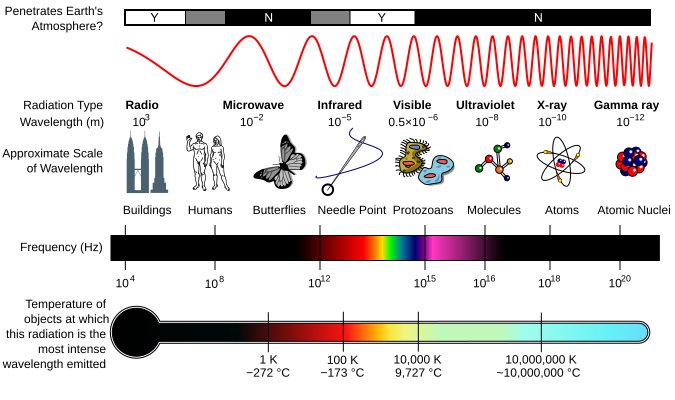
\includegraphics[width=\textwidth]{bilder/spektrum.png}
	\caption{Das elektromagnetische Spektrum mit Zuordnung typischer Anwendungen. Quelle: Wikimedia Commons}
	\label{fig:em_spektrum}
\end{figure}

\subsubsection{Frequenz-, Wellenlängen- und Energiebereiche}

\begin{table}[H]
	\centering
	\scriptsize
	\resizebox{0.95\textwidth}{!}{   % 0.95 = ca. 0,5 cm kleiner machen
		\begin{tabular}{|l|c|c|c|}
			\hline
			\textbf{\raisebox{-0.2ex}{Bereich}}& \textbf{\raisebox{-0.2ex}{Frequenz}}& \textbf{\raisebox{-0.2ex}{Wellenlänge}} &\textbf{\raisebox{-0.2ex}{Photonenenergie}}\\
			\hline
			Radiowellen      & \SI{1e3}{}–\SI{1e8}{Hz} & km – m & \(\sim\)\SI{1e-9}{eV} \\
			Mikrowellen      & \SI{1e8}{}–\SI{1e11}{Hz} & m – mm & \(\sim\)\SI{1e-6}{eV} \\
			Infrarot         & \SI{1e11}{}–\SI{4e14}{Hz} & mm – \SI{750}{nm} & \SI{1e-3}{eV} – \SI{1}{eV} \\
			Sichtbares Licht & \SI{4e14}{}–\SI{8e14}{Hz} & \SI{750}{nm} – \SI{380}{nm} & \SI{1.6}{eV} – \SI{3.3}{eV} \\
			Ultraviolett     & \SI{8e14}{}–\SI{3e16}{Hz} & \SI{380}{nm} – \SI{10}{nm} & bis \SI{100}{eV} \\
			Röntgen          & \SI{3e16}{}–\SI{3e19}{Hz} & \SI{10}{nm} – \SI{0.01}{nm} & \SI{100}{eV} – \SI{100}{keV} \\
			Gammastrahlung   & >\SI{3e19}{Hz} & < \SI{0.01}{nm} & > \SI{100}{keV} \\
			\hline
		\end{tabular}
	} % Ende resizebox
	\caption{Typische Bereiche des elektromagnetischen Spektrums mit Frequenz, Wellenlänge und Energie}
	\label{tab:spektrum}
\end{table}


\subsubsection{Einordnung von Anwendungen}

Typische Anwendungen in verschiedenen Spektralbereichen:

\begin{itemize}
	\item \textbf{Radiowellen:} Rundfunk, Funktechnik, MRT
	\item \textbf{Mikrowellen:} Mobilfunk, WLAN, Mikrowellenherd
	\item \textbf{Infrarot:} Fernbedienung, Thermografie
	\item \textbf{Sichtbar:} Optik, Fotografie, biologische Wahrnehmung
	\item \textbf{UV:} Sonnenbrand, Desinfektion (UV-C)
	\item \textbf{Röntgen:} Medizinische Bildgebung, Materialprüfung
	\item \textbf{Gamma:} Strahlentherapie, Astrophysik
\end{itemize}

\begin{tcolorbox}[hinweisbox,title=Fazit zum elektromagnetischen Spektrum]
	\label{box:Fazit zum elektro}
	\textbf{Physikalisches Fazit:}
	
	\begin{itemize}
		\item Das elektromagnetische Spektrum umfasst Wellen aller Frequenzen – von Radiowellen bis Gammastrahlen.
		\item Die Photonenenergie wächst mit zunehmender Frequenz (bzw. abnehmender Wellenlänge) gemäß \(E = h \nu = \frac{hc}{\lambda}\).
		\item Der Übergang zur \textbf{ionisierenden Strahlung} beginnt typischerweise im Bereich der UV-Strahlung, bei Photonenergien von etwa \SI{10}{\electronvolt}.
	\end{itemize}
	
	\vspace{0.5em}
	\textbf{Didaktisches Fazit:}
	
	\begin{itemize}
		\item Die Einordnung typischer Anwendungen – z.\,B. Mobilfunk, Mikrowelle, UV-Desinfektion oder Röntgendiagnostik – in das Spektrum erleichtert das Verständnis ihrer physikalischen und biologischen Wirkung.
		\item Besonders hilfreich ist die visuelle Verbindung zwischen Frequenz, Wellenlänge, Energie und biologischer Relevanz.
		\item \textbf{Merksatz:} Je kürzer die Wellenlänge, desto höher die Photonenenergie – und desto größer das Potenzial für biologische Schäden.
	\end{itemize}
\end{tcolorbox}
\newpage
\noindent
\subsection{Masselosigkeit und Bewegung mit \newline Lichtgeschwindigkeit}\index{Masselosigkeit}\index{Lichtgeschwindigkeit}

\subsubsection{Keine Ruhemasse -- aber Energie und Impuls}

Das Photon besitzt keine Ruhemasse, d.\,h. $m_0 = 0$. Dennoch ist es Tr\"ager von Energie und Impuls.\index{Energie} Die Energie eines Photons ergibt sich nach Planck und Einstein zu:
\begin{equation}
	E = h \nu
\end{equation}
Der Impuls eines Photons folgt daraus direkt:
\begin{equation}
	p = \frac{E}{c} = \frac{h\nu}{c} = \frac{h}{\lambda}
\end{equation}
Damit widerspricht das Photon nicht der Relativit\"atstheorie -- im Gegenteil: Diese Beziehungen sind genau die Konsequenz der speziellen Relativit\"at f\"ur masselose Teilchen.

\subsubsection{Was w\"are, wenn das Photon eine winzige Masse h\"atte?}

\paragraph{Relativistische Energieformel:} W\"are das Photon nicht ganz masselos, m\"usste man die allgemeine relativistische Energieformel verwenden:
\begin{equation}
	E = \gamma m_0 c^2 = \frac{m_0 c^2}{\sqrt{1 - \frac{v^2}{c^2}}}
\end{equation}
Dann g\"alte auch f\"ur den Impuls:
\begin{equation}
	p = \gamma m_0 v
\end{equation}
Die einfache Beziehung $E = pc$ w\"are dann nicht mehr korrekt, sondern es m\"usste gelten:
\begin{equation}
	E^2 = (pc)^2 + (m_0 c^2)^2
\end{equation}

(Eine mathematisch detaillierte Darstellung der Energie-Impuls-Relation für masselose und hypothetisch massive Photonen findet sich in Anhang~A, Abschnitt~\ref{anhangA:masse}.)
\newpage
\noindent
\subsubsection*{Physikalische Konsequenzen:}
\phantomsection
\begin{itemize}
	\item Die Lichtgeschwindigkeit w\"are nicht mehr konstant f\"ur alle Photonen.
	\item Die Geschwindigkeit h\"ange von der Energie (bzw. Frequenz) ab $\Rightarrow$ Verletzung der Lorentz-Invarianz.
	\item Langwelliges Licht w\"urde langsamer als kurzwelliges.
	\item Das Coulomb-Gesetz m\"usste modifiziert werden $\Rightarrow$ Reichweite der elektrischen Kraft endlich.
\end{itemize}

\paragraph{Experimentelle Grenzen:}
Pr\"azise Messungen zeigen: Wenn das Photon eine Masse besitzt, dann ist sie extrem klein:
\begin{equation}
	m_\gamma < 10^{-54} \text{ kg} \approx 10^{-18} \text{ eV}/c^2
\end{equation}
\index{Photonenmasse}

\textbf{Die Zahl} $10^{-54} \text{ kg}$ 	\textbf{ist kein Naturgesetz und auch kein theoretischer Wert}, sondern eine Obergrenze, die sich aus dem Ergebnis vieler Experimente und Beobachtungen ergibt – unter der Annahme, dass das Photon eine Masse haben könnte.
Solche winzigen Abweichungen konnten bisher nicht experimentell festgestellt werden.

\begin{figure}[H]
	\centering
	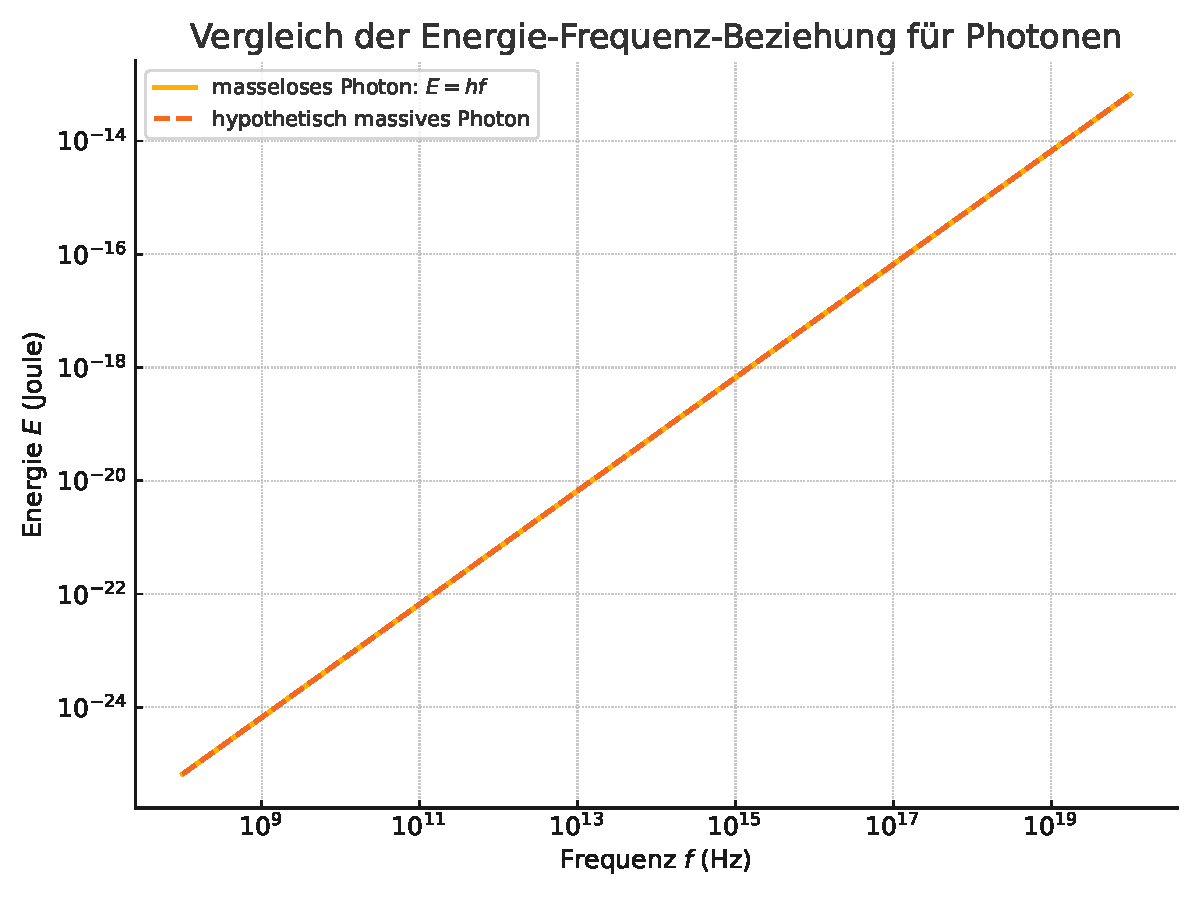
\includegraphics[width=0.85\textwidth]{bilder/photon_energie_vergleich_didaktisch.pdf}
	\caption{Didaktischer Vergleich der Energie-Frequenz-Beziehung \( E(f) \) für ein masseloses Photon (blau) und ein hypothetisch massives Photon mit überhöhter Masse (rot gestrichelt). }
	\label{fig:energie_f_masselos_massiv}
\end{figure}
\vspace{1em}
\begin{tcolorbox}[hinweisbox, title=Hinweis zur Grafik: Warum sieht man keinen Unterschied?]
	\label{box:Warum sieht man}
	Die Energie-Frequenz-Beziehung $E(f)$ wurde grafisch f\"ur masselose und hypothetisch massereiche Photonen dargestellt. Aufgrund der extrem kleinen experimentellen Obergrenze f\"ur die Photonenmasse ($m_\gamma < 10^{-54}$ kg) unterscheiden sich die beiden Kurven selbst im Log-Log-Diagramm praktisch nicht. \\[1ex]
	\textbf{Genau diese fehlende Abweichung ist ein starker Hinweis auf die Masselosigkeit des Photons.}
\end{tcolorbox}
\vspace{1em}
\begin{tcolorbox}[hypobox, title={Was wäre wenn, wenn das Photon eine Masse hätte? }]
	\label{box:was wäre wenn}
	Wenn das Photon eine auch nur winzige Masse hätte ($m_\gamma > 0$), dann:
	\begin{itemize}
		\item Würde es sich langsamer als Lichtgeschwindigkeit bewegen ($v < c$),
		\item Wäre die Energie-Frequenz-Beziehung nicht mehr $E = hf$, sondern:
		\begin{equation*}
			E = \sqrt{(hf)^2 + (m_\gamma c^2)^2}
		\end{equation*}
		\item Wäre die Lichtgeschwindigkeit nicht mehr konstant – z.\,B. würde langwelliges Licht langsamer laufen als kurzwelliges,
		\item Würde sich das Coulomb-Gesetz \textit{abschneiden} – die Reichweite elektrischer Felder wäre endlich.
	\end{itemize}
	Da all dies nicht beobachtet wird, gilt: Das Photon ist mit höchster Wahrscheinlichkeit wirklich masselos.
\end{tcolorbox}
\vspace{1em}
\newpage
\noindent
\subsubsection{Warum w\"urde \( E = h f \) bei massereichem Photon nicht mehr gelten?}

Die Formel $E = hf$ gilt nur exakt f\"ur masselose Teilchen. W\"are das Photon massereich, m\"usste gelten:
\begin{equation}
	E = \sqrt{(hf)^2 + (m_\gamma c^2)^2} > hf
\end{equation}
Die Energie hinge nicht mehr nur von der Frequenz ab -- und das w\"are experimentell messbar.

\paragraph{Best\"atigte Experimente:}
\begin{itemize}
	\item Photoeffekt
	\item Compton-Effekt
	\item Spektrallinien und Laserspektroskopie
	\item Quantenoptik und QED-Experimente
\end{itemize}
Alle best\"atigen mit hoher Pr\"azision die Beziehung $E = hf$. Eine systematische Abweichung wurde nie gefunden.
\vspace{1em}
\begin{tcolorbox}[physikbox, title=Fazit: Warum das Photon masselos ist]
	\begin{itemize}
		\label{box:Warum das Photon}
		\item Das Photon hat keine Ruhemasse ($m_0 = 0$), aber Energie und Impuls.
		\item Es bewegt sich zwingend mit Lichtgeschwindigkeit:\newline $v = c$.
		\item Nur unter dieser Bedingung gilt $E = pc$ und $E = hf$.
		\item W\"are $m_\gamma > 0$, w\"urde das gegen viele Beobachtungen und die spezielle Relativit\"at versto\"sen.
	\end{itemize}
\end{tcolorbox}
\vspace{1em}
\newpage
\noindent
\subsection{Spin und Polarisation}\index{Spin}\index{Polarisation}\index{Boson}\index{Helizität}

\subsubsection{Spin des Photons}

In der Quantenmechanik ist der \textbf{Spin} eine fundamentale Eigenschaft von Elementarteilchen – vergleichbar mit einem intrinsischen Drehimpuls. Anders als der klassische Drehimpuls bezieht sich der Spin nicht auf eine tatsächliche Rotation im Raum, sondern ist eine rein quantenmechanische Größe mit diskreten Werten.

\vspace{0.5em}
\textbf{Photonen besitzen den Spin 1}, gehören also zur Klasse der sogenannten \textit{Bosonen}. Während Teilchen mit halbzahligem Spin (wie Elektronen mit Spin $1/2$) den Fermionen zugeordnet werden und dem Pauli-Prinzip unterliegen, dürfen Bosonen denselben Quantenzustand einnehmen – ein Prinzip, das für Lichtteilchen fundamentale Konsequenzen hat, z.\,B. bei der Verstärkung von Laserlicht.\index{Fermion}\index{Pauli-Prinzip}\index{Laser}
\vspace{1em}
\begin{tcolorbox}[physikbox, title=Eigenschaften des Photon-Spins]
	\label{box:Eigenschaften des}
	\begin{itemize}
		\item Photonen haben \textbf{Spin 1}, aber keine Ruhemasse.
		\item Es gibt nur zwei messbare Spin-Zustände: \textbf{Helizität $+1$ und $-1$}.
		\item Die \textbf{Spinrichtung} liegt stets entlang der Bewegungsrichtung des Photons.
	\end{itemize}
\end{tcolorbox}
\vspace{1em}
Der Grund für die Beschränkung auf nur zwei Spin-Zustände liegt in der \textbf{Masselosigkeit des Photons}. Im Gegensatz zu massiven Spin-1-Teilchen (wie etwa dem Z-Boson) existiert für das Photon keine Ruhemasse, und somit auch kein Ruhesystem. Dadurch entfällt die Möglichkeit eines longitudinalen Spin-Zustands (Spin-0-Komponente), wie sie bei massiven Teilchen auftritt. Übrig bleiben nur die beiden Transversalmoden mit Helizität $\pm1$.\index{Z-Boson}

(Eine formale Herleitung der zulässigen Helizitätszustände des Photons findet sich in Anhang~A, Abschnitt~\ref{anhangA:helizitaet}.)

\newpage
\noindent
\textbf{Helizität} bezeichnet die Projektion des Spins auf die Bewegungsrichtung des Teilchens. Für Photonen bedeutet dies:
\begin{itemize}
	\item \textbf{Helizität $+1$}: Rechtszirkular polarisiertes Licht.
	\item \textbf{Helizität $-1$}: Linkszirkular polarisiertes Licht.
\end{itemize}

\begin{figure}[H]
	\centering
	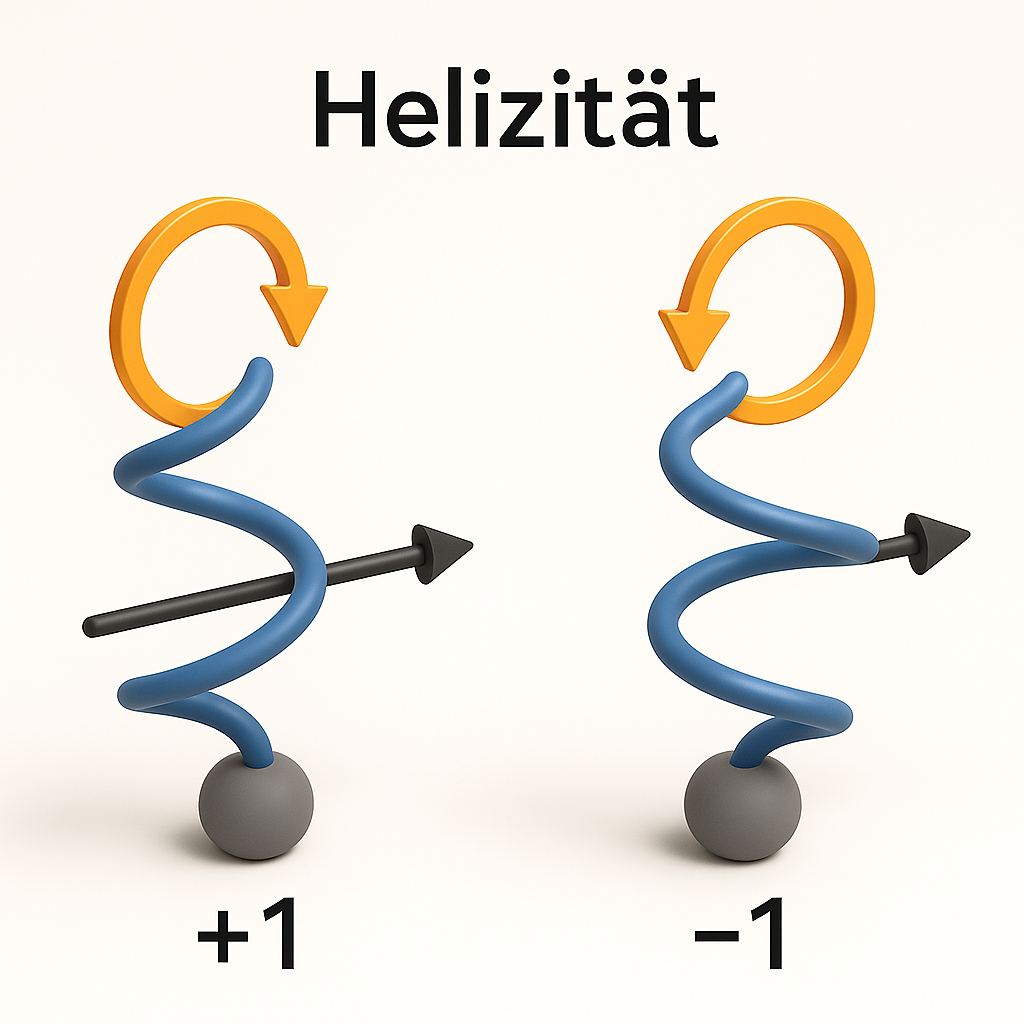
\includegraphics[width=0.65\textwidth]{bilder/Helizitaet.png}
	\caption{Visualisierung der Helizität eines Photons. Links: Helizität $+1$ (rechtszirkular), rechts: Helizität $-1$ (linkszirkular). Die orangefarbenen Pfeile zeigen die Drehrichtung (Spin), die schwarzen Pfeile die Ausbreitungsrichtung des Photons.}
	\label{fig:helizitaet}
\end{figure}

\begin{tcolorbox}[physikbox, title=Kommentar zur Darstellung]
	\label{box:Kommentar zur Darstellung}
	Die spiralförmige Struktur veranschaulicht, wie sich der elektrische Feldvektor bei zirkular polarisierter Strahlung dreht. Das Photon bewegt sich geradlinig entlang der Ausbreitungsrichtung (Impulspfeil). Die gezeigte Spirale stellt die Rotation des Feldes dar – nicht den Flugweg. Dies ist eine wichtige Unterscheidung beim Verständnis von Helizität.
\end{tcolorbox}
\vspace{1em}
Diese beiden Zustände bilden die quantenmechanische Grundlage für die \textit{zirkulare Polarisation}, auf die wir im nächsten Abschnitt näher eingehen.

\newpage
\noindent
Zum Vergleich:
\begin{itemize}
	\item Ein \textbf{Elektron} besitzt Spin $1/2$ mit zwei Zuständen (up/down).
	\item Ein \textbf{Z-Boson} (massiv, Spin 1) zeigt drei Zustände: $-1$, $0$, $+1$.
	\item Das \textbf{Photon} (masselos, Spin 1) zeigt nur $-1$ und $+1$ – der $0$-Zustand entfällt.
\end{itemize}
\vspace{1em}
\begin{tcolorbox}[physikbox, title=Didaktischer Merksatz]
	\label{box:didaktischerMerksatz}
	Masselose Spin-1-Teilchen wie Photonen besitzen nur zwei mögliche Helizitätszustände: \textbf{$\pm1$}. Der longitudinal gepolte Zustand mit $0$ existiert nicht, weil sich kein Ruhesystem definieren lässt.
\end{tcolorbox}
\vspace{1em}
\subsubsection*{Fazit}
\phantomsection
Der Spin des Photons unterscheidet sich grundlegend vom Spin massiver Teilchen. Als masseloses Spin-1-Teilchen besitzt das Photon nur zwei mögliche Helizitätszustände: +1 und -1. Ein longitudinaler Spin-Zustand mit Helizität 0 ist ausgeschlossen, da kein Ruhesystem existiert.

\vspace{0.5em}
Die Rotation des Spins kann daher nur entlang der Bewegungsrichtung betrachtet werden – sie äußert sich in der Helizität:

\begin{itemize}
	\item Helizität +1: Spin zeigt in Bewegungsrichtung (rechtszirkular)
	\item Helizität -1: Spin zeigt entgegen der Bewegungsrichtung (linkszirkular)
\end{itemize}

Der klassische Begriff einer realen Rotation ist hier nicht anwendbar. Der Spin ist eine intrinsische quantenmechanische Eigenschaft, die sich beim Photon als zirkulare Polarisation zeigt.

\subsubsection{Polarisation als makroskopische Erscheinung \newline des Spins}

Die Polarisation von Licht ist ein beobachtbares Phänomen, das direkt mit dem quantenmechanischen Spin des Photons verknüpft ist. Während der Spin eine intrinsische Eigenschaft jedes einzelnen Photons darstellt, beschreibt die Polarisation den kollektiven Zustand eines Lichtfeldes – also vieler Photonen gemeinsam.

\vspace{0.5em}
Klassisch versteht man unter Polarisation die Ausrichtung des elektrischen Feldvektors einer elektromagnetischen Welle. Dieser schwingt stets senkrecht zur Ausbreitungsrichtung, kann jedoch verschiedene Richtungen und Rotationen annehmen:

\begin{itemize}
	\item \textbf{Linear polarisiertes Licht:} Der elektrische Feldvektor schwingt in einer festen Richtung (z.\,B. vertikal oder horizontal).
	\item \textbf{Zirkular polarisiertes Licht:} Der elektrische Feldvektor rotiert mit konstanter Amplitude im Kreis – im Uhrzeigersinn (rechtszirkular) oder gegen den Uhrzeigersinn (linkszirkular).
	\item \textbf{Elliptisch polarisiertes Licht:} Allgemeinster Fall – der Feldvektor beschreibt eine Ellipse.
\end{itemize}
\index{Linear polarisiertes Licht}\index{Zirkular polarisiertes Licht}\index{Elliptisch polarisiertes Licht}

\vspace{0.5em}
In der Quantenoptik entspricht die Polarisation dem kollektiven Zustand der Helizitäten vieler Photonen.\index{Quantenoptik} Ein vollständig rechtszirkular polarisiertes Lichtfeld besteht aus Photonen mit Helizität +1, linkszirkular polarisiertes Licht aus Photonen mit Helizität -1. Lineare Polarisation entsteht aus einer quantenmechanischen Überlagerung beider Zustände:

\begin{equation}
	|\text{linear}\rangle = \frac{1}{\sqrt{2}} \left( |+1\rangle + |-1\rangle \right)
\end{equation}

(Eine ausführlichere Darstellung der Polarisation in der Dirac-Notation und mit Jones-Vektoren findet sich in Anhang~A, Abschnitt~\ref{anhangA:polarisation}.)
\vspace{1em}
\begin{tcolorbox}[physikbox, title=Superposition und Polarisation]
	\label{box:Superposition}
	Ein linear polarisiertes Photon ist ein quantenmechanischer Überlagerungszustand der beiden Helizitätszustände $|+1\rangle$ und $|-1\rangle$. Diese Superposition führt zur festen Schwingungsrichtung des elektrischen Feldes.
\end{tcolorbox}

\vspace{0.5em}
Damit stellt die Polarisation eine direkt beobachtbare Konsequenz des Photon-Spins dar. In vielen Experimenten – z.\,B. mit Polarisationsfiltern, Polarisationskameras oder im Doppelspaltversuch mit polarisierter Strahlung – zeigt sich die Polarisation als makroskopisch messbares Phänomen quantenmechanischer Ursprünge.\index{Polarisationsfilter}
\vspace{1em}
\begin{tcolorbox}[physikbox, title=Superposition und Polarisation]
	\label{box:Superposition und Polarisation}
	Ein linear polarisiertes Photon befindet sich in einem quantenmechanischen Überlagerungszustand der beiden Helizitätszustände $|+1\rangle$ (rechtszirkular) und $|-1\rangle$ (linkszirkular):
	
	\[
	|\text{linear}\rangle = \frac{1}{\sqrt{2}} \left( |+1\rangle + |-1\rangle \right)
	\]
	
	Diese Superposition bedeutet:
	\begin{itemize}
		\item Das Photon besitzt keine definierte Helizität.
		\item Es ist gleichzeitig in den Zuständen $|+1\rangle$ und $|-1\rangle$ – mit gleicher Amplitude und fester Phasenlage.
		\item Die feste Schwingungsrichtung (lineare Polarisation) entsteht durch diese kohärente Überlagerung.
		\item Eine Messung der Helizität zerstört den Superpositionszustand: Das Photon wird entweder mit Helizität $+1$ oder $-1$ nachgewiesen – aber nie in beiden Zuständen zugleich.
	\end{itemize}
	
	Diese Darstellung zeigt: Polarisation ist mehr als eine Richtung des elektrischen Feldes – sie ist Ausdruck eines quantenmechanischen Zustands, der sich erst durch Superposition vollständig beschreiben lässt.
\end{tcolorbox}

\subsubsection{Messung und Nachweis der Polarisation}

Die Polarisation des Lichts ist eine makroskopisch beobachtbare Konsequenz der quantenmechanischen Spinstruktur von Photonen. Um sie experimentell zu untersuchen, stehen verschiedene optische Verfahren zur Verfügung – von einfachen Polarisationsfiltern bis hin zu präzisen Einzelphotonen-Detektoren in der Quantenoptik.

\vspace{0.5em}
\textbf{Lineare Polarisation} lässt sich klassisch mit Polarisationsfiltern nachweisen: Ein linear polarisiertes Lichtbündel wird durch einen zweiten Filter („Analysator“) geschickt. Je nach Drehwinkel zwischen beiden Filtern variiert die Intensität nach dem \textbf{Malus’schen Gesetz}:\index{Malus’sches Gesetz}

\[
I = I_0 \cos^2\theta
\]

Dabei ist \( \theta \) der Winkel zwischen Polarisationsrichtung des einfallenden Lichts und der Filterachse. Dieser Zusammenhang liefert einen direkten experimentellen Zugriff auf die Polarisationsebene.

\vspace{0.5em}
\textbf{Zirkulare Polarisation} kann durch Kombination eines linearen Polarisationsfilters mit einer Viertelwellenplatte sichtbar gemacht werden.\index{Viertelwellenplatte} Diese wandelt zirkulare Polarisation in lineare um, die dann analysiert werden kann.

\vspace{0.5em}
\textbf{Einzelphotonen-Experimente} in der Quantenoptik ermöglichen den direkten Nachweis quantisierter Polarisation:
\begin{itemize}
	\item Ein Photon trifft auf einen Polarisator. Es wird entweder durchgelassen oder absorbiert.
	\item Wiederholte Messungen an gleichpräparierten Photonen ergeben statistisch die Polarisation.
	\item Diese Experimente zeigen: Polarisation ist ein Einzelphotonenphänomen, keine rein klassische Wellenerscheinung.
\end{itemize}

\vspace{0.5em}
\textbf{Technische Anwendungen} der Polarisation sind zahlreich:
\begin{itemize}
	\item LCD-Bildschirme, Polarisationsbrillen, Fernerkundung
	\item Kommunikation durch Polarisationsmultiplex (z./,B. in der Glasfasertechnik)
	\item Quantenkommunikation mit polarisierten Einzelphotonen (QKD)
\end{itemize}
\index{QKD (Quantenkryptographie)}\index{Polarisationsmultiplex}

\begin{tcolorbox}[physikbox, title=Was uns die Polarisation über Photonen verrät ]
	\label{box:Was uns die}
	Polarisation ist nicht nur eine Eigenschaft elektromagnetischer Wellen, sondern ein direkt messbares Resultat des quantenmechanischen Spins von Photonen. Durch Polarisationsmessungen lassen sich fundamentale Aussagen über den Zustand einzelner Lichtquanten treffen – bis hin zur Verschränkung in der Quantenphysik.
\end{tcolorbox}
\index{Verschränkung}

\subsection{Fazit }\index{Fazit}

Kapitel~III hat gezeigt, wie sich das Licht aus quantenmechanischer Sicht nicht nur als elektromagnetische Welle, sondern auch als Teilchen -- das Photon -- verstehen lässt. Dieses Verständnis vereint klassische Konzepte wie Frequenz und Polarisation mit quantisierten Eigenschaften wie Energie, Impuls und Spin.

\vspace{0.5em}
Zentrale Erkenntnisse:
\begin{itemize}
	\item Die Energie eines Photons ist direkt proportional zur Frequenz: \( E = h\nu \).
	\item Der Impuls eines Photons ergibt sich aus seiner Wellenlänge: \( p = \frac{h}{\lambda} \).
	\item Photonen besitzen Spin~1, zeigen aber aufgrund ihrer Masselosigkeit nur die Helizitätszustände +1 und -1.
	\item Die Polarisation makroskopischer Lichtfelder ist ein kollektives Phänomen, das sich auf die quantenmechanischen Zustände vieler Photonen zurückführen lässt.
\end{itemize}

\vspace{0.5em}
Diese quantisierten Eigenschaften des Photons werden in Kapitel~IV eine zentrale Rolle spielen, wenn wir die Wellennatur von Teilchen und den Teilchencharakter von Wellen in Form des Welle-Teilchen-Dualismus betrachten.
